\begin{figure}[t]
\centering
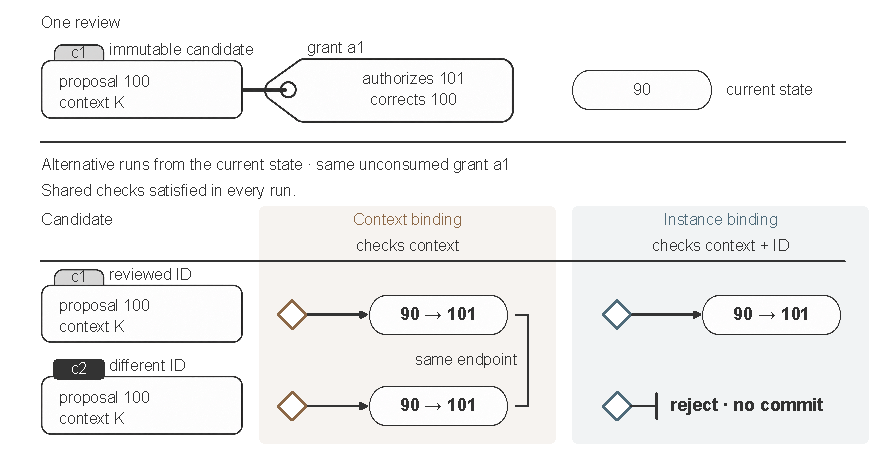
\includegraphics[width=\linewidth]{figures/fig1-review-execution-gap.pdf}
\caption{Equal endpoints do not identify the reviewed instance. A reviewer corrects candidate c1's proposal 100, and grant a1 authorizes 101 for c1. Candidate c2 carries the same proposal and retained context $K$ but a different identifier. Each path represents an alternative execution from the current state 90 with the original grant a1 still unconsumed and the shared checks satisfied. Diamonds mark checks, capsules show the initial state or committed transitions, and the stop bar marks no commit. Context binding admits either candidate and installs 101; instance binding admits only c1. A matching new authorization could license c2, subject to the shared checks. The four roles are the machine proposal (100), the authorized correction (101), the reviewed candidate (c1), and the executed transition ($90 \to 101$). This is a conceptual construction. Object glyphs were AI-generated; see the AI-assisted preparation declaration}
\label{fig:gap}
\end{figure}
